\documentclass[letterpaper]{article}

\usepackage{amsmath}
\usepackage{gensymb}
\usepackage[vmargin=1in,hmargin=1.25in]{geometry}
\usepackage{graphicx}
\usepackage{hyperref}
\usepackage{microtype}
\usepackage{lmodern}
\usepackage{tikz}
\usetikzlibrary{matrix}

\author{Philip Pham}
\title{\Large ECE/CSE 576, Spring 2019 Homework 3: Content-Based Image Retrieval}
\date{\today}

\begin{document}
\maketitle

\section{Algorithm}

For each image, we performed $k$-means clustering with $k = 8$ for 32
iterations.\footnote{A random seed of 2020 was used for reproducibility.}
Connected components was then applied to segment the image into contiguous
regions. For each region, the following features were computed: (1) the
proportion of the image occupied the region, (2) the average red, green, and
blue color levels scaled to lie in range $[0,1]$, (3) the centroid, (4) the
bounding box, and (5) a normalized gray-level co-occurence matrix (GLCM).

For the centroid and bounding box, coordinates were scaled to lie in range
$[0, 1]$. The gray-levels were binned into 8 buckets each of size 32. The
neighboring pixel of $(r, c)$ was the diagonal pixel at
$\left(r^\prime = r + 1, c^\prime = c + 1\right)$.

\subsection{Distance 1}

Distance 1 was simply the squared Euclidean distance over the 5 classes of
features:
\begin{equation}
  d_1\left(\mathbf{x}, \mathbf{y}\right) = \left\lVert \mathbf{x} - \mathbf{y}\right\rVert_2^2.
  \label{eqn:distance_1}
\end{equation}
For the vectors in Equation \ref{eqn:distance_1}, the first coordinate is the
volume, the colors are the next 3 entries, the centroid are the next 2 entries
in the vector, the top, right, bottom, and left of the bounding box make the
next 4 entries, and the normalized GLCM are the last 64 entries for a total of
74 features.

\subsection{Distance 2}

The secod distance function is more complex and uses several derived features.
\begin{equation}
  d_2\left(\mathbf{x}, \mathbf{y}\right) = 
  \label{eqn:distance_2}
\end{equation}

\section{Results}

\subsection{\texttt{Beach}}
\begin{center}
  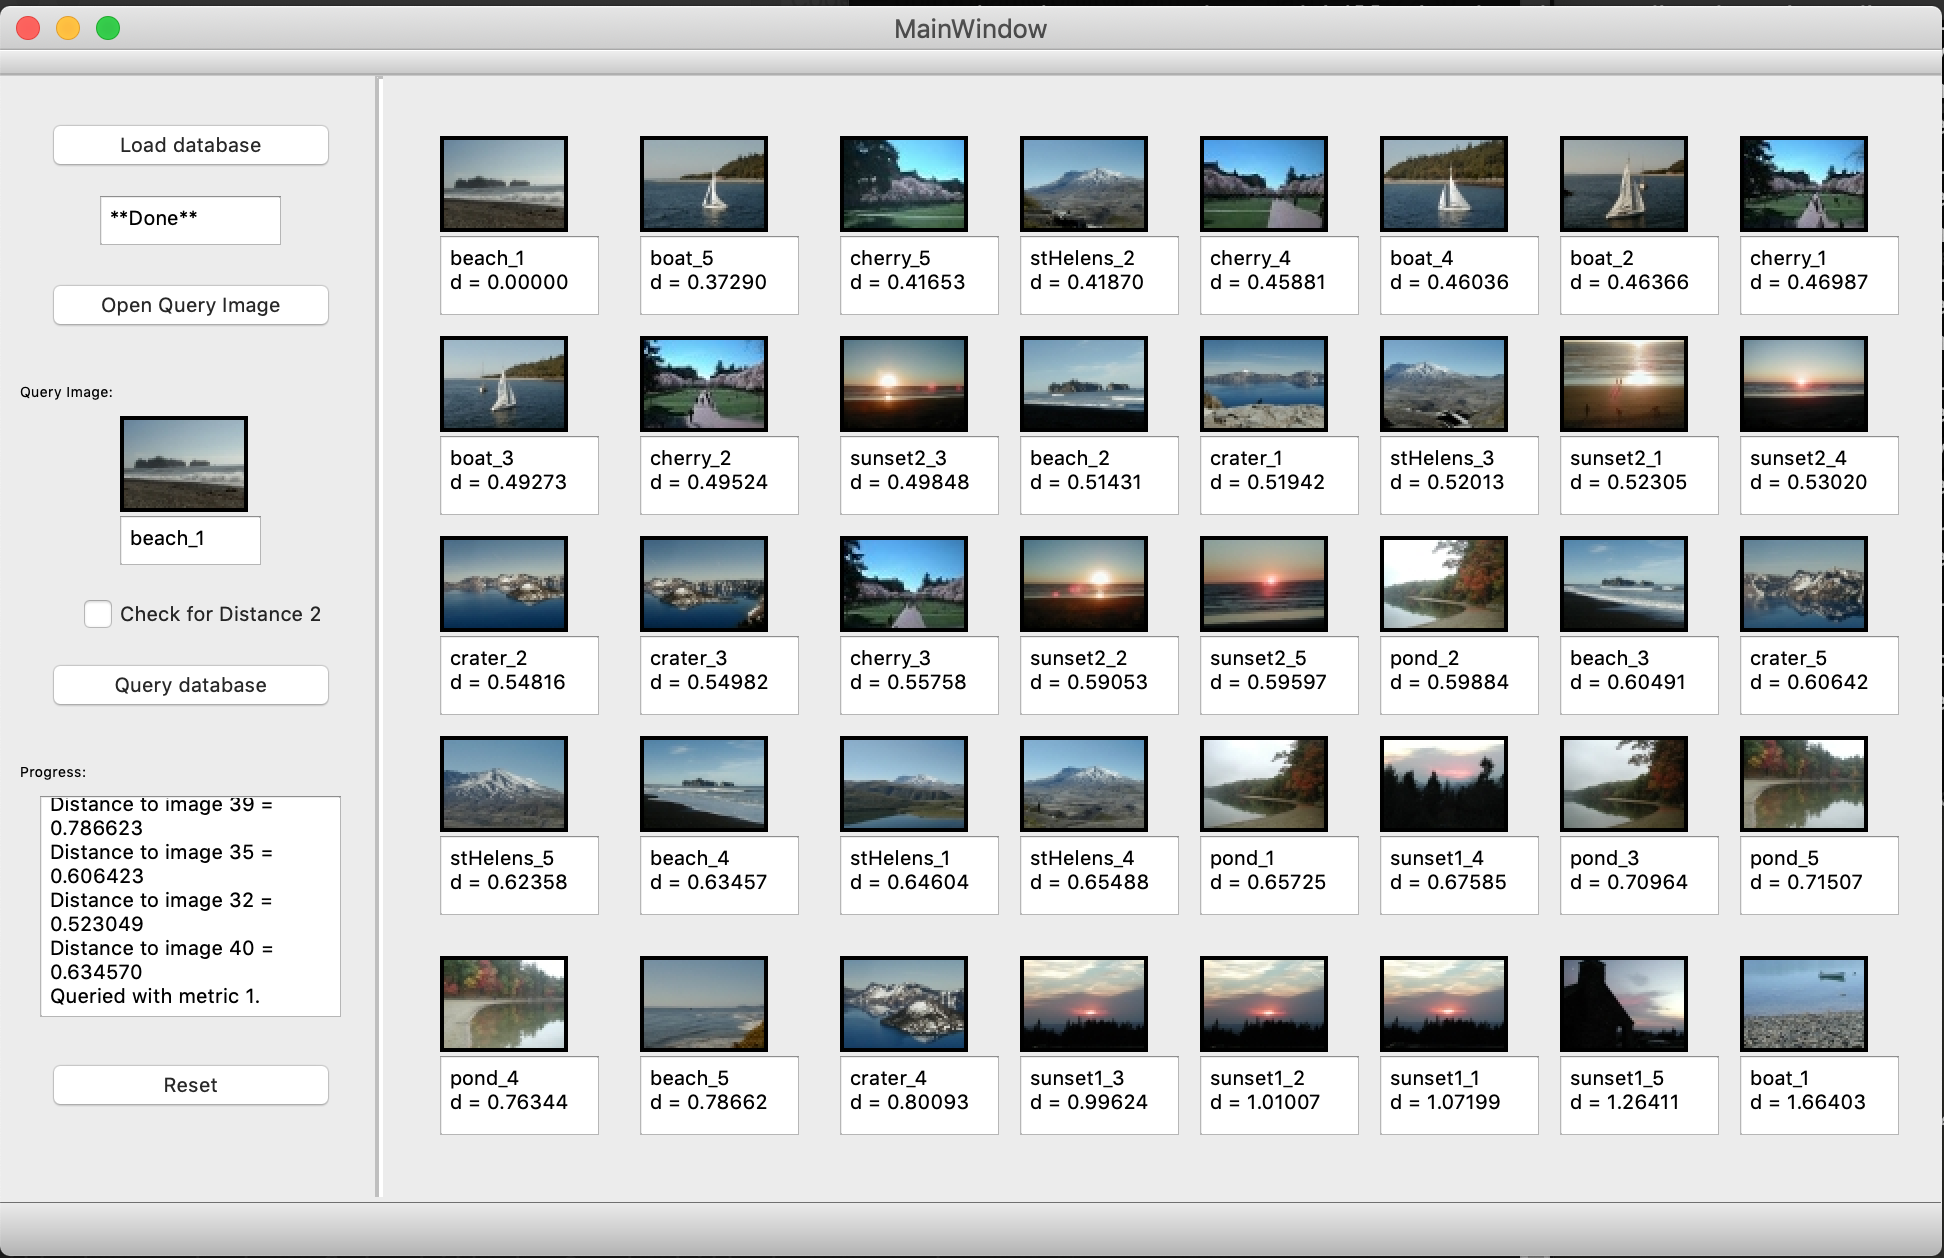
\includegraphics[width=\textwidth]{beach_1_distance1.png}
  
  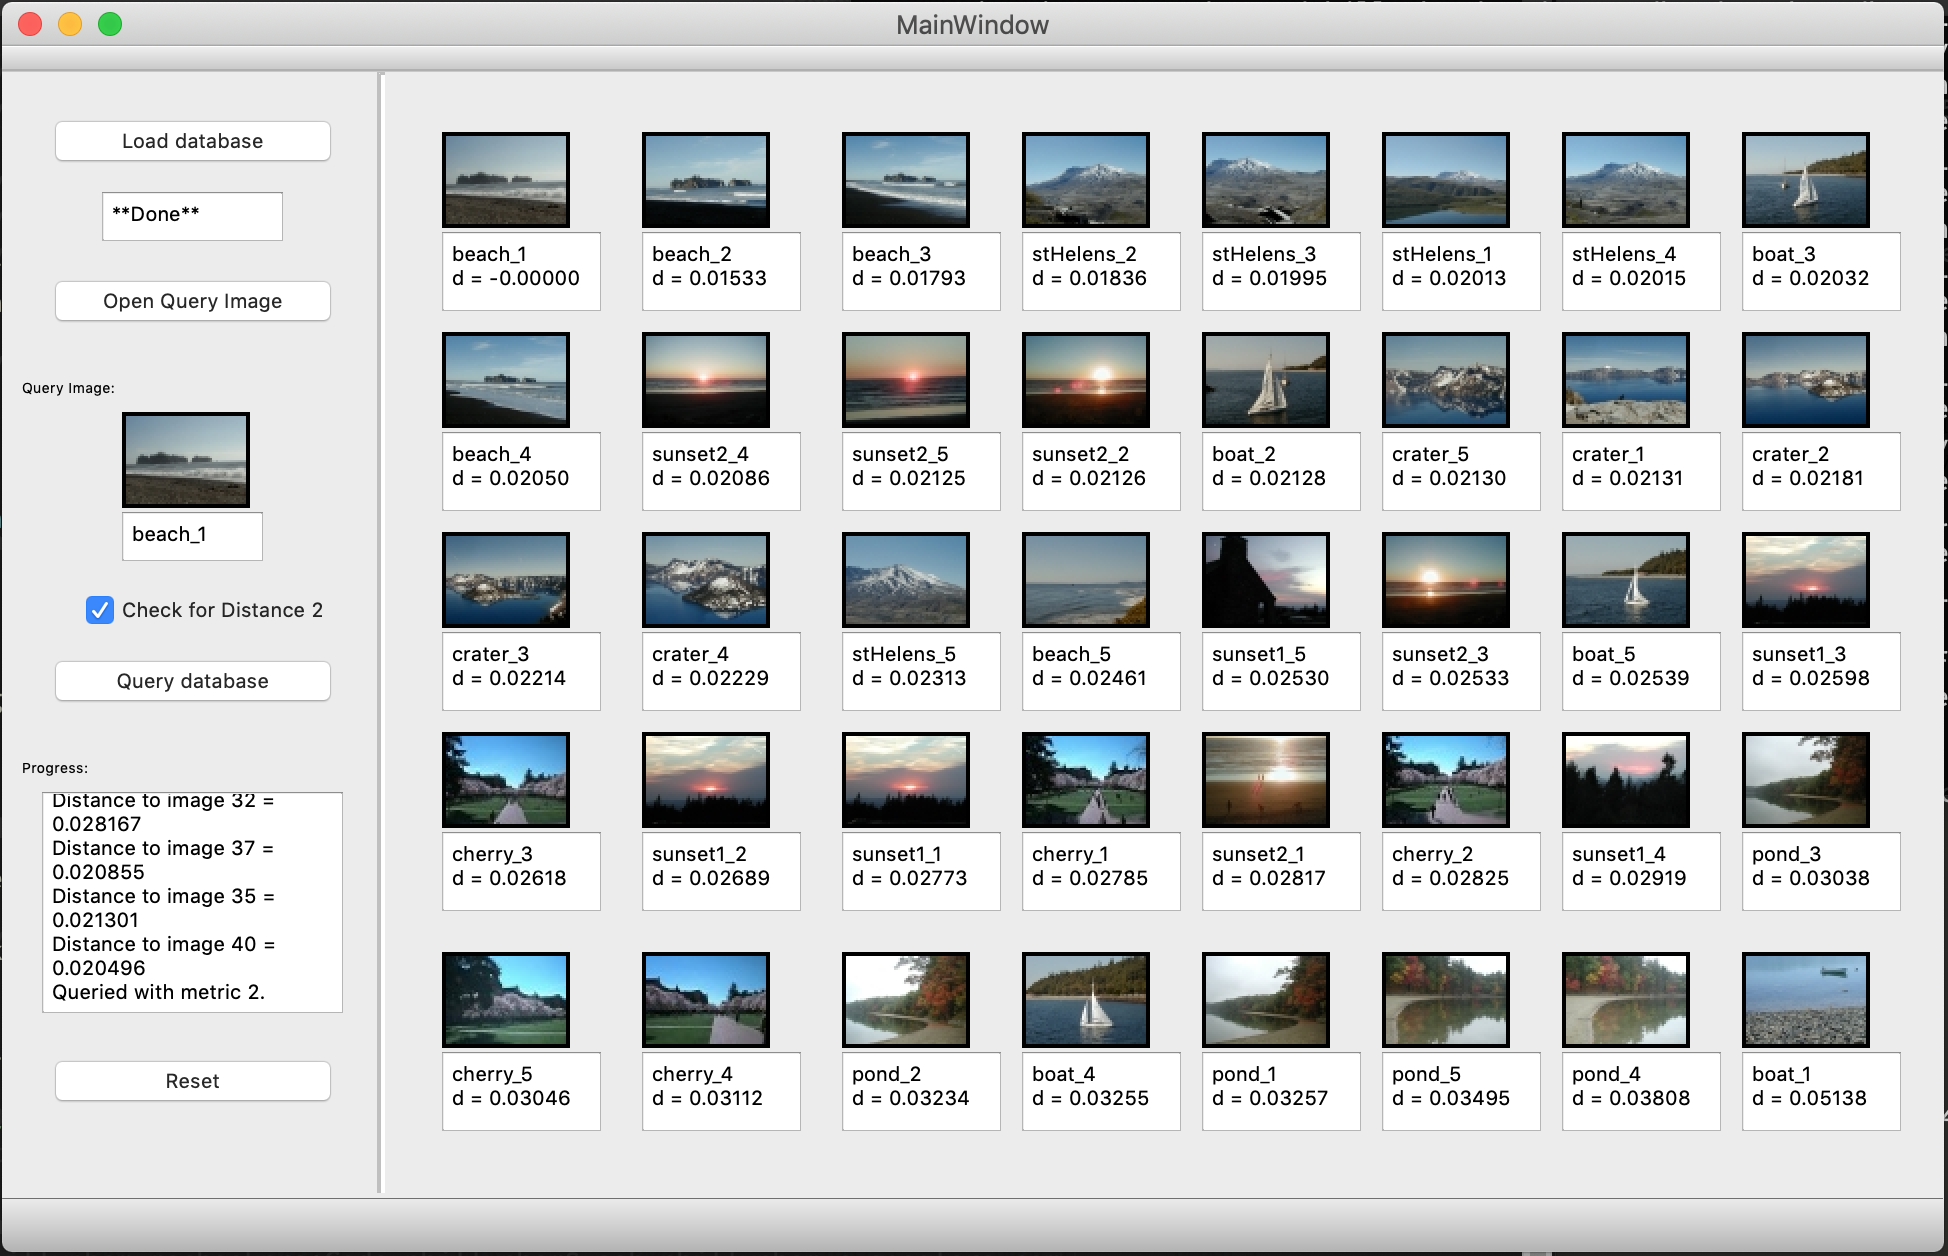
\includegraphics[width=\textwidth]{beach_1_distance2.png}
  
  Query results for \texttt{beach\_1.jpg}.
\end{center}

The beach queries proved challenging. Euclidean distance completely fails, while
$d_2$ only manages to return $2/4$ beach images.

\subsection{\texttt{Boat}}
\begin{center}
  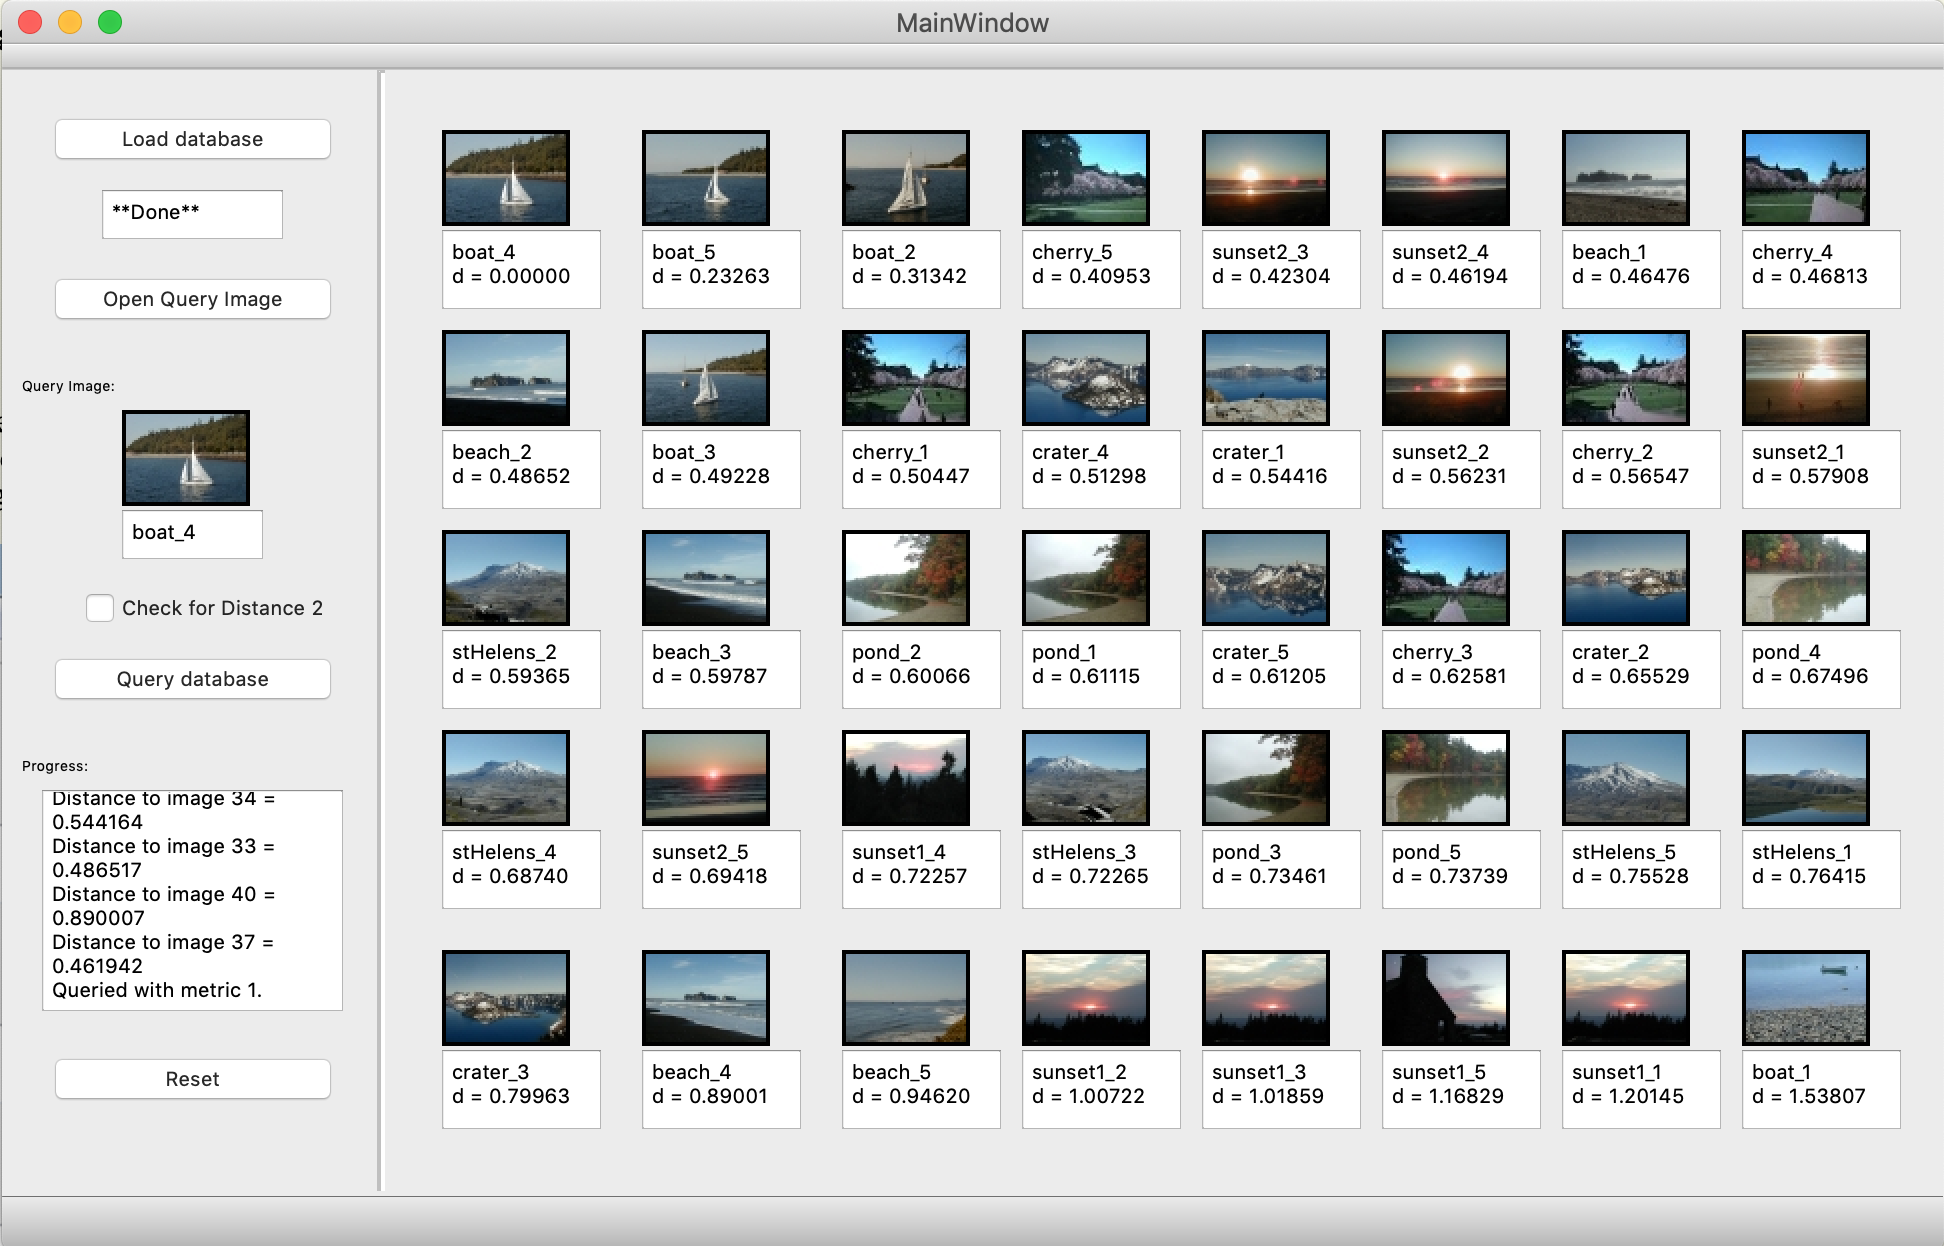
\includegraphics[width=\textwidth]{boat_4_distance1.png}
  
  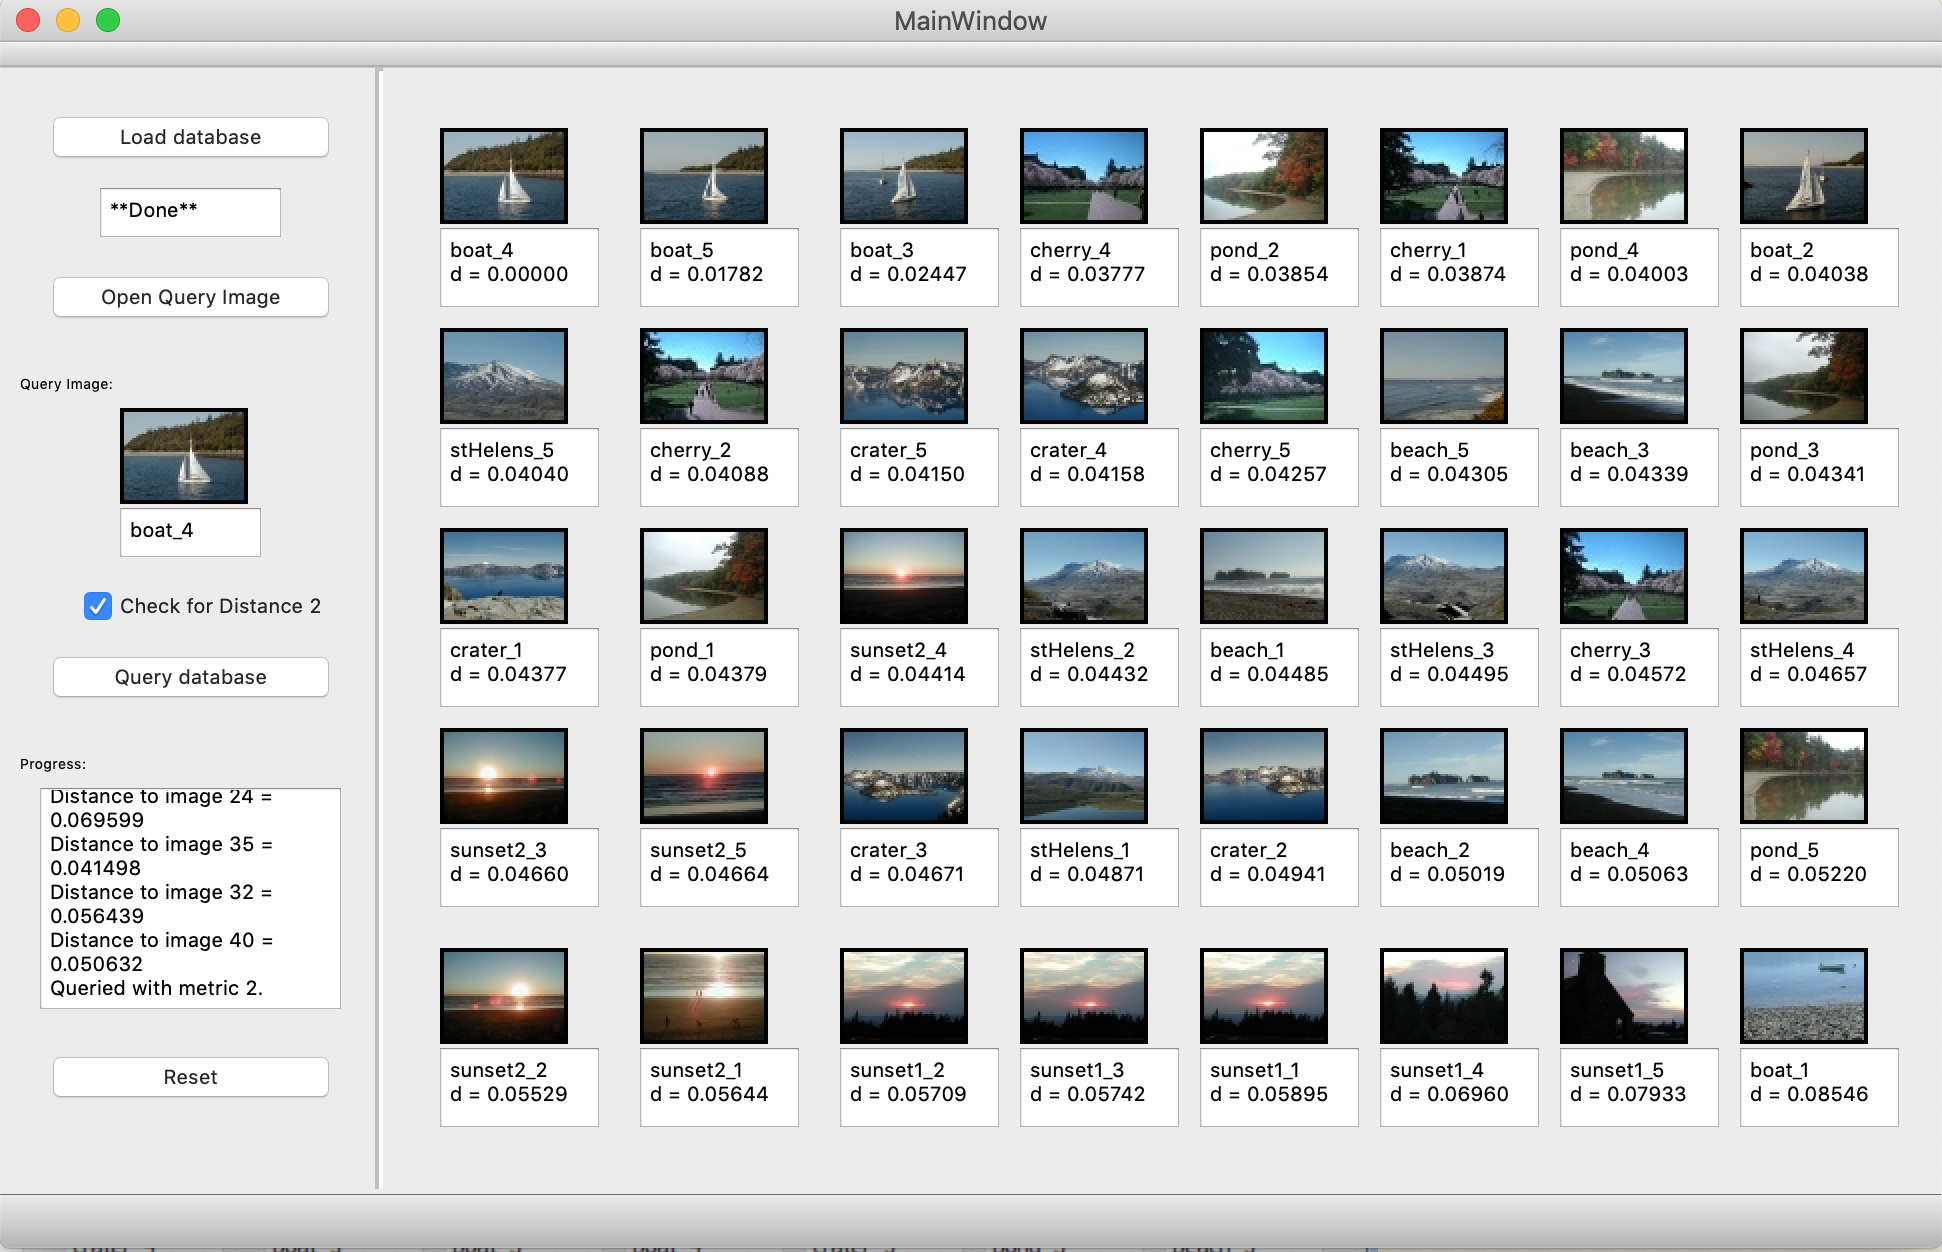
\includegraphics[width=\textwidth]{boat_4_distance2.png}
  
  Query results for \texttt{boat\_4.jpg}.
\end{center}

$d_1$ and $d_2$ both return other boat images for their top two results. One
might say that $d_2$ does slightly better since it has another boat result in
the top row.


\section*{Appendix}

All code used to generate these images can be found at
\href{https://github.com/ppham27/cse576/blob/master/hw3}{\texttt{ppham27/cse576/hw3}}. The
embedded JPEG, PNG files, and the \LaTeX can be found in
\href{https://github.com/ppham27/cse576/blob/master/hw3/report}{\texttt{ppham27/cse576/hw3/report}}.

\end{document}
